\section{Fourier-Transformation}
	\subsection{Berechnungen}%
		\begin{tabular}{|p{6cm} l|} \hline
			\textbf{Fouriertransformierte:} &
			$F(j\omega) = \int\limits_{-\infty}^{\infty} f(t)e^{-j\omega t}dt$ \\
			\textbf{Rücktransformierte:} &
			$f(t) = \frac{1}{2\pi}\int\limits_{-\infty}^{\infty}F(j\omega)e^{j\omega t}d\omega$ \\ \hline
		
		Dies ergibt das \textbf{Korespondenzpaar:} & $f(t) \; \laplace \; F(\omega)$ \\
		mit der \textbf{Symetrie:} & $F(t) \; \laplace \; 2\pi \cdot f(-\omega)$ \\
		
		$F(\omega) = R(\omega) -jX(\omega)$ wobei: ($f(t)$ reell!) &
		$R(\omega) = \int\limits_{-\infty}^\infty f(t)\cdot \cos(\omega t)\,dt \quad\quad X(\omega) =
		\int\limits_{-\infty}^\infty f(t)\cdot \sin(\omega t)\,dt$
		\\
		&$f(t)$ gerade: $X(\omega)$ verschwindet, f(t) ungerade: $R(\omega)$ verschwindet \\
		\hline
		\end{tabular}
		
		f sei stückweise stetig $\frac{1}{2}(f(t^+) + f(t^-)) = \frac{1}{2\pi} \int\limits_{-\infty}^{\infty}F(\omega)e^{j\omega t} dt$
		
		Jede reelle $f(t)$ lässt sich aus Summe einer geraden und einer ungeraden Funktion beschreiben:\\
		\begin{tabular}{lll}
		$f(t) = f_e(t) + f_o(t)$ mit & $f_e(t) = \frac{1}{2}[f(t) + f(-t)]$ & $f_o(t) = \frac{1}{2}[f(t) - f(-t)]$ \\
		
		Also: & $R(\omega) = 2 \int\limits_0^\infty f_e(t) \cos(\omega t)\,dt$ & $X(\omega) = 2 \int\limits_0^\infty
		f_o(t) \sin(\omega t)\,dt$ \\
		
		Und: & $f_e(t) = \frac{1}{\pi}\int\limits_0^\infty R(\omega)\cos(\omega t)\,d\omega$ & 
		$f_o(t) = \frac{1}{\pi}\int\limits_0^\infty X(\omega)\sin(\omega t)\,d\omega$ \\
		\end{tabular}
		
		Bei \textbf{kausalen} Funktionen gilt:\\
		\begin{tabular}{c c c}
			$f(t) = 0$ falls $t<0$ & 
			$f_e(t) = f_o(t) = \frac{1}{2}f(t)$ &
			$f(t) = \frac{2}{\pi}\int\limits_0^\infty R(\omega) \cos(\omega t)\,dt = \frac{2}{\pi}\int\limits_0^\infty X(\omega) \sin(\omega t)\,dt$
		\end{tabular}
			
		\begin{tabular}{|l|l|l|}
		\hline
		Spektraldichte / Spektraldarstellung	& $F(\omega)$ 		& KEINE absoluten Werte für Amplitude \& Phase \\
		\hline
		Amplitudendichte 						& $|F(\omega)| $		& f reell $\rightarrow$
		$|F(\omega)|$ symetrisch zur Ordinatenachse
		\\
		\hline
		Phasendichte							& $arg(F(\omega))$	& f reell $\rightarrow$ $arg(F(\omega))$ punktsymetrisch zum Ursprung \\
		\hline
		Kosinusamplitudendichte					& $R(\omega)$		& f reell $\rightarrow$ $R(\omega)$ gerade \\
		\hline
		Sinusamplitudendichte					& $X(\omega)$ 		& f reell $\rightarrow$ $X(\omega)$ ungerade \\
		\hline
		Amplitudengang				& $A(\omega) = |H(\omega)|$ & $= \sqrt{H(\omega)\cdot \overline{H(\omega)}} \qquad$ 
		
		$\begin{cases}
			< 1 \text{ Dämpfung}\\
			> 1 \text{ Verstärkung}
		\end{cases}$ \\
		& & $\overline{H(\omega)}$ bilden durch +/- Tausch vor j-Term  \\
		\hline
		Dämpfung & $\dfrac{1}{A(\omega)} = \left|\dfrac{1}{H(\omega)}\right|$ &  \\ 
		\hline
		Phasenverschiebung						& $\Phi(\omega) = arg(H(\omega))$ & $= \arctan\left( \dfrac{Im(H(\omega))}{Re(H(\omega))}\right)$ \\
		\hline
		Systemantwort							& $H(\omega) = A(\omega) \cdot e^{\jmath \Phi(\omega)}$ & \\
		\hline
		\end{tabular}
		
		\subsection{Symmetrie}
			Es gelten die gleichen Symmetrien wie bei der Fourierreihe.
				
				
		\subsection{Eigenschaften}
					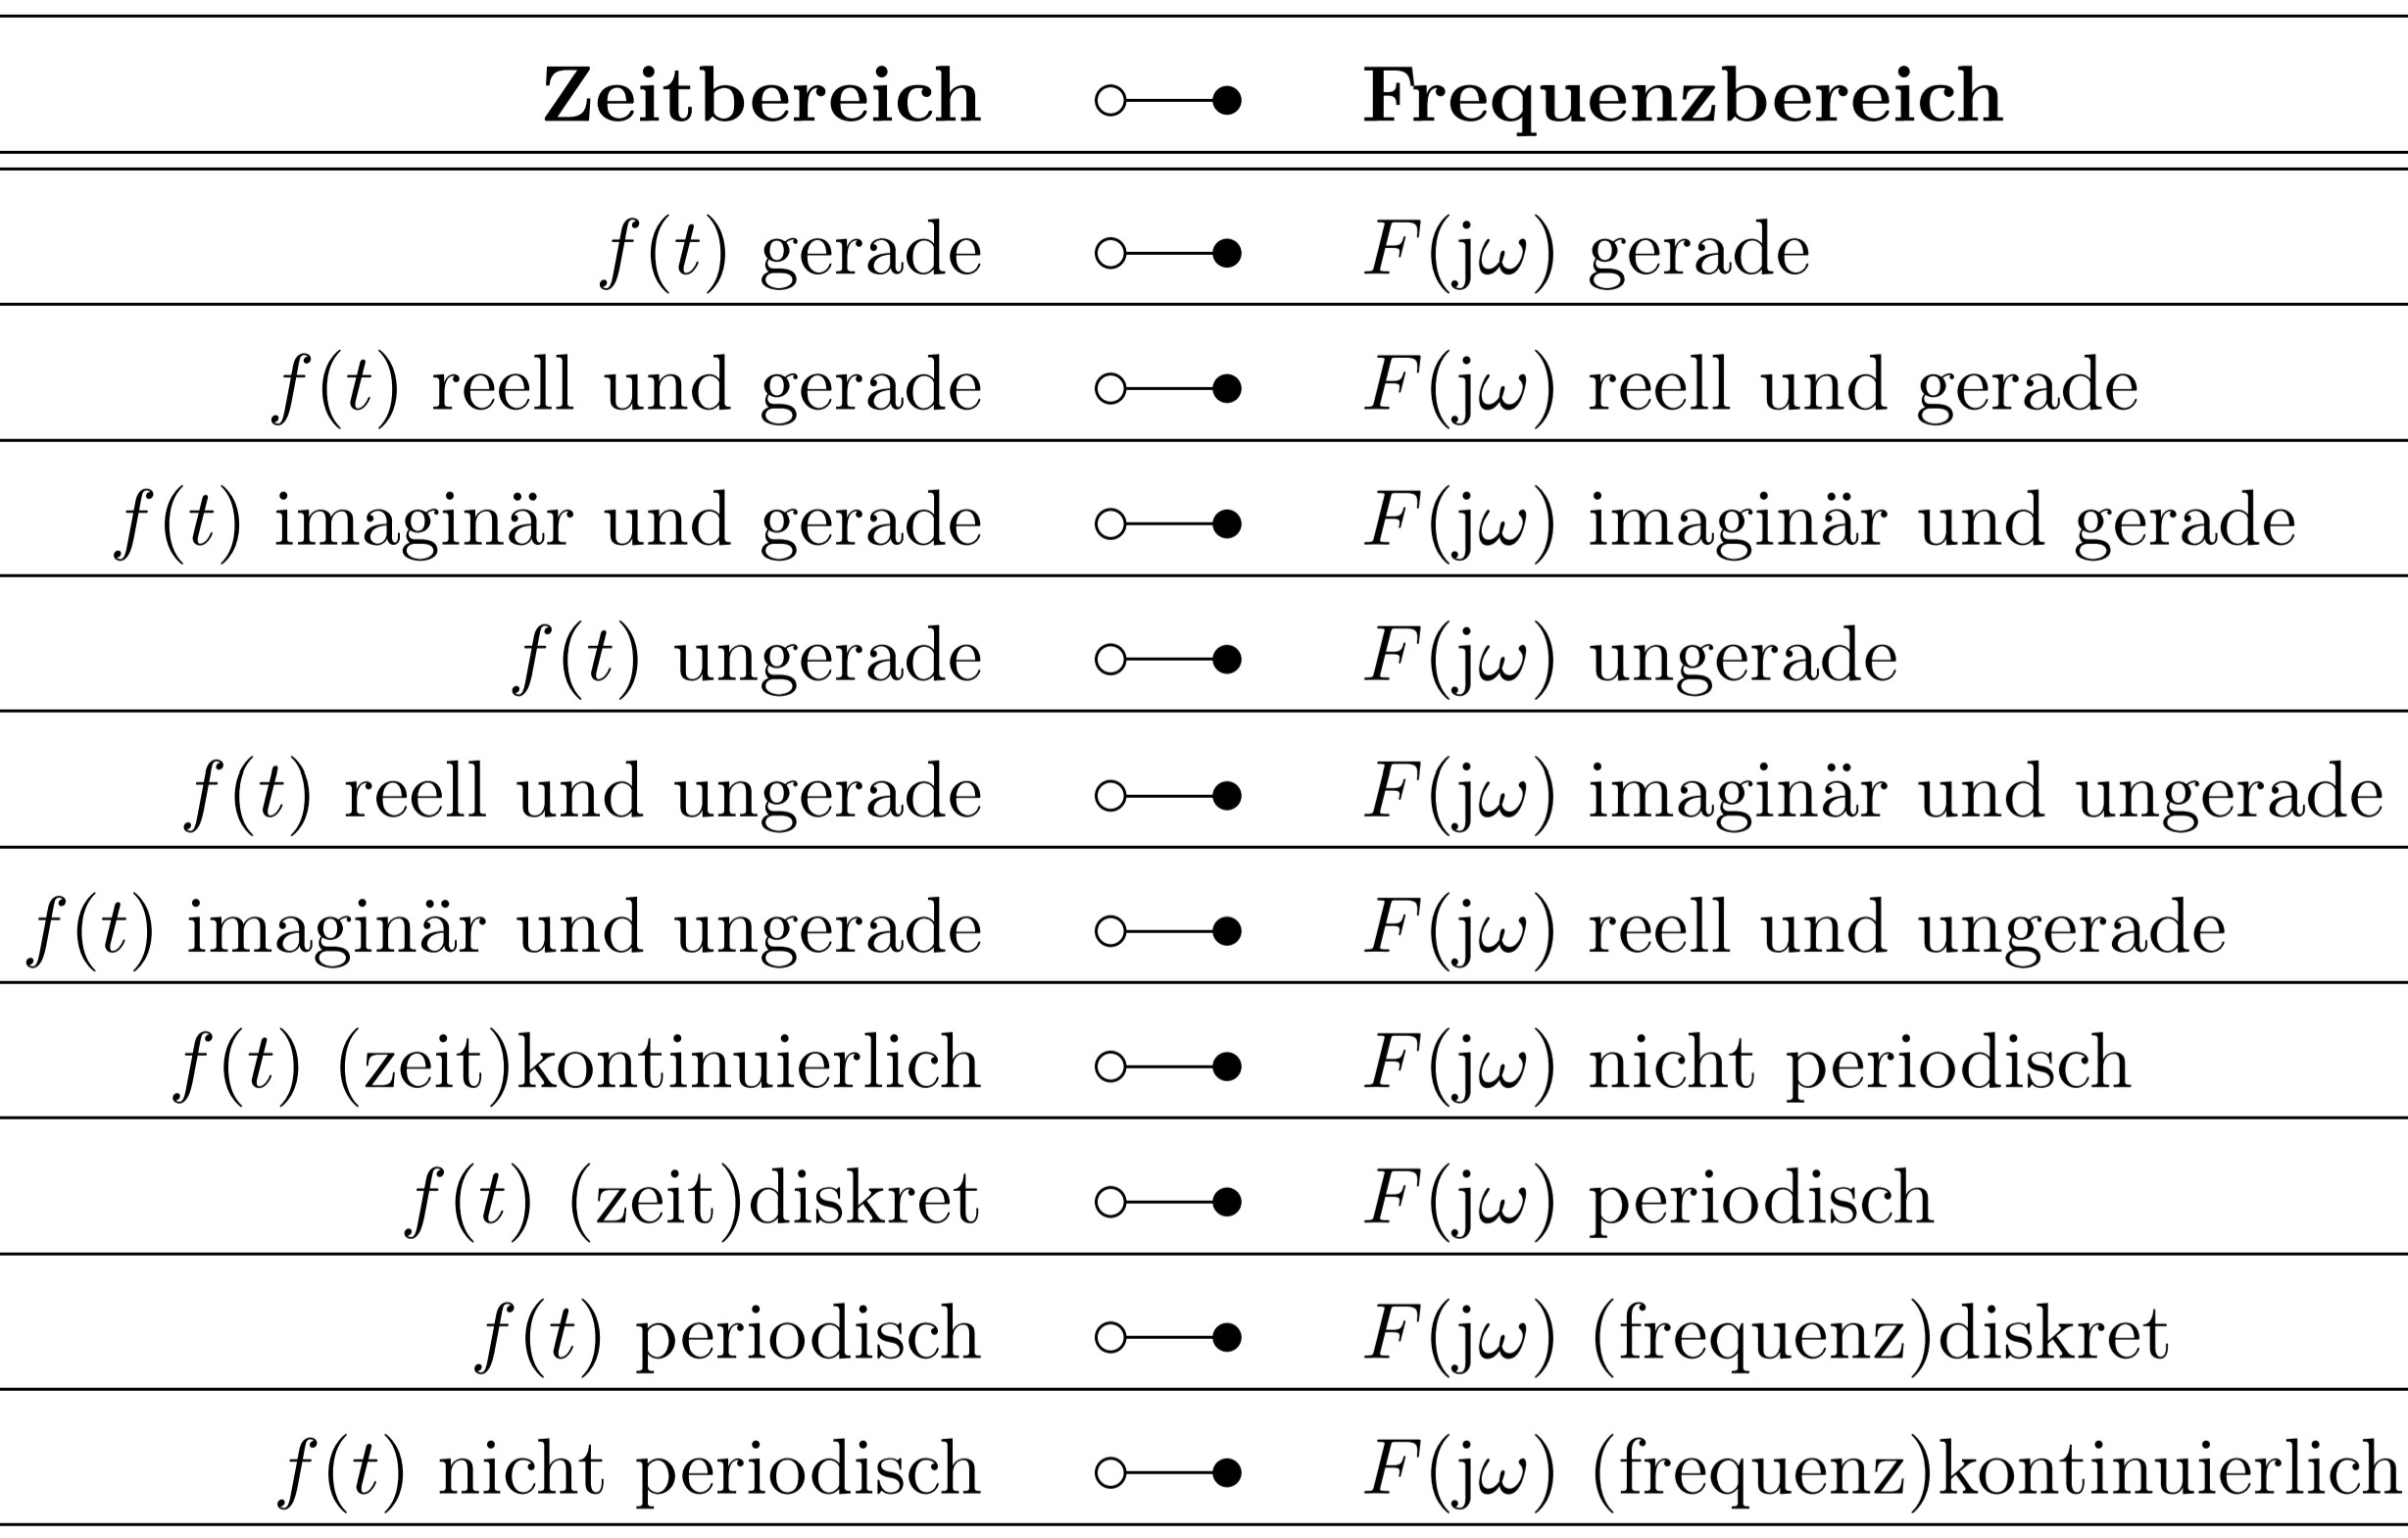
\includegraphics[width=10cm]{./bilder/EigenschaftenFT.jpg}\\
					
				\begin{tabular}{|p{9cm}|p{8cm}|}
		        	\hline
			        	Linearität & 
			        	$\alpha\cdot f(t) + \beta\cdot g(t) \; \laplace \; \alpha\cdot F(\omega) +
			        	\beta\cdot G(\omega)$\\
		        	\hline
						Zeitumkehrung (Spiegelung an der Y-Achse)&
						$f(-t) \; \laplace \; F(-\omega) = F^*(w)$ \\
					\hline        	
			  			"Ahnlichkeit / Zeitskalierung &
			  			$f(\alpha t) \; \laplace \; \frac{1}{|\alpha|}F \left (\frac{\omega}{\alpha} \right)
			  			\quad\alpha \in\mathbb{R}\setminus \{0\}$\\
							& $F(\alpha\omega) \; \Laplace \; f(\frac{t}{\alpha})$ \\
		  			\hline
		  			\hline
			  			Verschiebung im	Zeitbereich &
			  			$f(t\pm t_0) \; \laplace \; F(\omega)e^{\pm j\omega t_0}$\\
		  			\hline
						Verschiebung im Frequenzbereich (Modulationstheorem) &
						$f(t)e^{\pm j\omega_0 t} \; \laplace \; F(\omega\mp\omega_0)$\\
					\hline
					\hline
						Ableitung im Zeitbereich &
						$\frac{\partial^n f(t)}{\partial t^n} \; \laplace \; (j\omega)^n F(\omega) \qquad (n \in \mathbb{N}_0)$\\
					\hline				
						Ableitung im Frequenzbereich &
						$t^n f(t) \; \laplace \; j^n \frac{\partial F(\omega)}{\partial \omega^n}$\\
					\hline
					\hline		
						Faltung im Zeitbereich &
						$f(t) \ast g(t) = \int\limits_{-\infty}^{\infty} f(\tau)g(t-\tau)d\tau \; \laplace \;
						F(\omega) \cdot G(\omega)$\\
					\hline
						Faltung im Frequenzbereich &
						$f(t) \cdot g(t) \; \laplace \; \frac{1}{2\pi}F(\omega) \ast G(\omega)$\\
					\hline
					\hline
						Integration im Zeitbereich &
						$\int\limits_{-\infty}^{t}f(\tau)d\tau \; \laplace \;
						\frac{F(\omega)}{j\omega}+F(0)\pi\delta(\omega)$\\
					\hline
						Vertauschungssatz (Dualität) &
						$f(t) \; \laplace \; F(\omega)\nonumber$ \\
			 			& $F(t) \; \laplace \; 2\pi \cdot f(-\omega)$\\
		 			\hline
			 			Modulation &
			 			$\cos(\alpha t) \cdot f(t)  \; \laplace \;  \frac{1}{2}\cdot
			 			\left[F(\omega-\alpha) + F(\omega+\alpha)\right ]$\\
			 			& $\sin(\alpha t) \cdot f(t) \; \laplace \; \frac{1}{2j}\cdot \left[
			 			F(\omega-\alpha) - F(\omega+\alpha)\right ]$\\
		 			\hline
			        	Parseval's Theorem &
			 			$\int\limits_{-\infty}^{\infty}f(t)g^{\ast}(t)dt = \frac{1}{2\pi}
			  			\int\limits_{-\infty}^{\infty}F(\omega)G^{\ast}(\omega)d\omega$\\
		  			\hline
			  			Bessel's Theorem &
			  			$\int\limits_{-\infty}^{\infty}|f(t)|^2 dt = \frac{1}{2\pi}
			  			\int\limits_{-\infty}^{\infty}|F(\omega)|^2 d\omega$\\
		  			\hline 			
						Anfangswerte &
						$f(0)=\frac{1}{2\pi}\int\limits_{-\infty}^{\infty}F(\omega)d\omega
						\hspace*{1cm} F(0)=\int\limits_{-\infty}^{\infty}f(t)dt$\\
					\hline
						$\infty$ lange Folge von $\delta$-Impulsen &
						$\sum_{n=-\infty}^{\infty} \delta(t-n\cdot t_0) \; \laplace \;
						\sum_{n=-\infty}^{\infty} \frac{2\pi}{t_0}\delta(\omega-n\cdot
						\frac{2\pi}{t_0})$\\
					\hline
		     \end{tabular}
		     
	
		\subsubsection{Wichtige Fouriertransformierten-Paare}
			\includegraphics[width=0.7\textwidth]{./bilder/fourierTransPaare.png}\\		